
\documentclass[11pt]{article}
\usepackage[a4paper,margin=1in]{geometry}
\usepackage{fontspec}
\usepackage{setspace}
\usepackage{microtype}
\usepackage{booktabs}
\usepackage{longtable}
\usepackage{array}
\usepackage{tabularx}
\usepackage{ragged2e}
\usepackage{xcolor}
\usepackage{tikz}
\usetikzlibrary{arrows.meta,positioning,shapes.geometric,shapes.misc,calc,matrix,fit}
\usepackage[hidelinks]{hyperref}
\usepackage{caption}
\usepackage{enumitem}
\setmainfont{Times New Roman}
\onehalfspacing
\emergencystretch=3em
\setlength{\parskip}{0.45em}
\setlength{\parindent}{1.2em}
\definecolor{camblue}{HTML}{1F4E79}
\definecolor{softblue}{HTML}{DCEAF7}
\definecolor{softgreen}{HTML}{DDEFEA}
\definecolor{softyellow}{HTML}{F8E7C1}
\definecolor{softred}{HTML}{EFD4CC}
\definecolor{softgray}{HTML}{ECEFF1}
\definecolor{boxborder}{HTML}{2F3A45}
\title{From Neural Machine Translation to LLM-Augmented Translation Workflows: A Scoping Survey}
\author{Xiongfei Wang\\[0.3em]\begin{minipage}{0.86\textwidth}\centering
Faculty of English Language and Culture, Guangdong University of Foreign Studies, Guangzhou, China, 510420\\
Email: \href{mailto:pencinus@qq.com}{pencinus@qq.com}\\
ORCID: \href{https://orcid.org/0009-0005-9560-6420}{0009-0005-9560-6420}
\end{minipage}}
\date{}
\begin{document}
\maketitle
\noindent\textbf{Article type:} Survey Paper\\
\textbf{Running title:} LLM-Augmented Translation Workflows\\
\textbf{Corresponding author:} Xiongfei Wang, \href{mailto:pencinus@qq.com}{pencinus@qq.com}\\
\textbf{ORCID:} \href{https://orcid.org/0009-0005-9560-6420}{0009-0005-9560-6420}

\begin{abstract}
This Survey Paper maps how neural machine translation (NMT), Transformer-based systems, and large language models (LLMs) are being integrated into translation workflows. Although LLMs are often discussed as direct translators, the emerging literature suggests a broader and more consequential role: LLMs increasingly function as post-editors, evaluators, error explainers, terminology controllers, document-level context handlers, translation-memory users, and human-facing assistants. We conducted a PRISMA-ScR-informed scoping survey of studies published or made available between 2017 and 2026, with a final extraction corpus of forty-eight full-review records and seven background or exclusion records. The corpus was coded by model type, workflow stage, language pair, domain, dataset, evaluation method, human involvement, and reproducibility indicators. The review identifies six major evidence clusters: LLMs as post-editors of NMT output; LLMs as translation-quality evaluators; terminology, style, domain, and low-resource control; document-level and multimodal translation; human-centred translation workflows; and fairness, hallucination, robustness, and safety. Across these clusters, the central finding is that the field is moving from model-centred translation quality comparisons toward workflow-level questions about reliability, cognitive ergonomics, terminology governance, reproducibility, and accountability. However, evidence remains uneven. Professional CAT-tool deployments, privacy and confidentiality in real translation workflows, longitudinal studies of trust and productivity, high-stakes legal and medical MTPE, and prompt-level reproducibility are still underdeveloped. We propose a workflow-oriented taxonomy and a research agenda for evaluating LLM-augmented translation systems as socio-technical translation infrastructures rather than isolated text generators.
\end{abstract}

\noindent\textbf{Keywords:} machine translation; large language models; post-editing; translation quality evaluation; human-centred NLP

\section{Introduction}
Machine translation has long been one of the central applications of natural language processing. The field has moved from phrase-based statistical systems to neural sequence-to-sequence models, attention-based NMT, Transformer architectures, massively multilingual systems, and most recently LLM-based translation and translation assistance. This history matters because current debates about LLMs in translation are often framed too narrowly. The question is frequently posed as whether ChatGPT, GPT-4, Gemini, Llama, or another generative model is a better translator than a conventional NMT system. That question is important, but it is not sufficient.

In practical translation settings, translation is rarely a single-step act of generating a target sentence from a source sentence. Professional, educational, and institutional translation workflows can include project preparation, terminology and style management, translation-memory retrieval, draft generation, interactive correction, post-editing, quality estimation, error annotation, client-side review, and risk management. LLMs can enter the workflow at many of these points. They may generate a first draft, but they may also revise NMT output, explain errors, produce MQM-style annotations, adapt terminology, retrieve examples, support translator training, or simulate an evaluator. The unit of analysis therefore needs to shift from the isolated system output to the translation workflow.

This survey takes that workflow view. It asks how NMT and LLMs are being combined across translation tasks and what the evidence shows about their roles, limitations, and evaluation practices. The survey is motivated by three observations. First, recent LLM translation research is highly fragmented across ACL, WMT, EAMT, AMTA, HCI, translation studies, education, and applied AI venues. Second, many studies evaluate outputs with automatic metrics, while fewer measure translator effort, trust, cognitive load, or domain-specific risk. Third, the most distinctive contributions of LLMs often appear outside direct translation: in post-editing, evaluation, context handling, explanation, adaptation, and interaction.

The contribution of this paper is threefold. First, we provide a scoping map of NMT and LLM research across translation workflow stages. Second, we synthesize the main evidence clusters and show how they reshape the research problem from translation quality alone to workflow quality. Third, we propose a research agenda for LLM-augmented translation that foregrounds reproducibility, human-centred evaluation, low-resource language equity, terminology governance, fairness, hallucination, privacy, and professional accountability.

This positioning distinguishes the present survey from two adjacent kinds of review. Context-oriented NMT surveys clarify discourse, document-level modelling, and context evaluation, but they do not treat LLMs as workflow components across post-editing, evaluation, terminology, human interaction, and risk governance (Castilho and Knowles 2024). Recent MT-and-LLM surveys provide a broader historical and model-centred account of translation in the LLM era, but they give less attention to the operational question of how LLMs are inserted into translation pipelines and what evidence is available for each role (Ataman et al. 2025). The present survey is therefore deliberately narrower in one sense and broader in another: it is narrower because it does not aim to catalogue all MT or LLM translation research, but broader because it treats translation as a staged workflow involving models, resources, evaluators, human translators, and institutional accountability.


The workflow framing also helps distinguish two kinds of novelty that are sometimes conflated. A model may be novel because it improves a standard MT benchmark, but a workflow may be novel because it changes the distribution of work among an MT engine, a large language model, a translation memory, a human translator, and a quality-control procedure. The second form of novelty is harder to evaluate, because it depends on interaction, institutional constraints, and risk tolerance. It is nevertheless central to translation technology. Many professional translation tasks are not won by the most fluent isolated sentence; they are won by reliable handling of constraints across many segments, consistent reuse of client terminology, documented revision, and accountability for the final text.

The LLM moment has intensified this issue because general-purpose models can be inserted into nearly every stage of the workflow. A prompt can ask the model to translate, explain, compare, rewrite, classify, detect errors, produce an MQM label, apply a glossary, adapt to a style guide, or justify a revision. These capabilities make LLMs attractive to researchers and practitioners, but they also blur role boundaries. If the same model drafts a translation and evaluates the draft, the apparent evaluation may partly reflect model self-preference. If the model post-edits NMT output without transparent instructions, improvements may come with hidden additions or stylistic drift. If a model is used as an assistant for translators, productivity gains may depend on expertise, trust calibration, and the cost of monitoring plausible but wrong output.

This paper therefore treats LLM-augmented translation as a socio-technical NLP problem. The technical system includes models, prompts, retrieval resources, decoding settings, benchmarks, and metrics. The social and professional system includes translators, reviewers, clients, language communities, institutional confidentiality requirements, domain specialists, and end users. A survey that ignores either side will miss the central question: not only whether LLMs can translate, but under what workflow conditions they can be trusted to support translation.


\section{Background and methods}
\subsection{From NMT to LLM-augmented translation technology}
NMT established the modern neural framing of translation as sequence transduction. Early attention-based encoder-decoder models showed that a single neural architecture could learn to align and translate jointly (Bahdanau et al. 2015). Production-scale NMT systems, including GNMT, demonstrated that neural systems could substantially improve fluency and adequacy in deployed translation services (Wu et al. 2016). The Transformer then replaced recurrent architectures with self-attention and became a central architecture for both NMT and later LLMs (Vaswani et al. 2017).

The post-Transformer period brought two related but distinct trajectories. One trajectory scaled multilingual NMT. NLLB-200 expanded translation coverage to two hundred languages, with particular attention to low-resource languages, human evaluation, toxicity measurement, and data quality (NLLB Team et al. 2024). SEAMLESSM4T extended this trajectory into speech and text, supporting speech-to-speech, speech-to-text, text-to-speech, and text-to-text translation across many languages while also evaluating noise, gender bias, and added toxicity (Seamless Communication et al. 2025). These systems remain important background for LLM-based translation because they show that translation quality is shaped by data curation, multilingual transfer, evaluation design, safety filtering, and deployment constraints.

The second trajectory is the rise of general-purpose LLMs. Unlike task-specific encoder-decoder MT systems, LLMs can be prompted, fine-tuned, or used in multi-step workflows. Their general linguistic and reasoning capabilities make them attractive for translation-related tasks that require explanation, adaptation, or interaction. However, the same generality introduces instability: outputs may depend on prompt phrasing, model version, decoding settings, context length, and undocumented training data. For translation, this creates a tension between flexibility and control.

Recent surveys have begun to describe the historical and technical relationship between MT and LLMs (Ataman et al. 2025). The present paper differs by treating LLMs not only as new translation engines, but as components in translation workflows. This distinction aligns with the literature we reviewed: LLMs are used to post-edit NMT, evaluate translation quality, generate error spans, tune terminology, incorporate translation memories, support low-resource prompting, handle document context, augment multimodal data, and interact with human translators.

The background literature also shows why traditional NMT should remain part of the survey rather than being treated as obsolete. Transformer NMT created the architectural and evaluative environment in which LLM translation now operates. Metrics, datasets, shared tasks, terminology constraints, low-resource transfer, and document-level evaluation all have pre-LLM histories. Many current LLM studies compare against NLLB, Google Translate, DeepL, mBART, or other NMT systems. These comparisons are not merely baselines; they show which parts of the translation workflow were already well served by specialised MT and which parts are newly opened by general-purpose language models.

Figure 1 summarises the major conceptual turning points used to frame the review.

\begin{figure}[t]
\centering
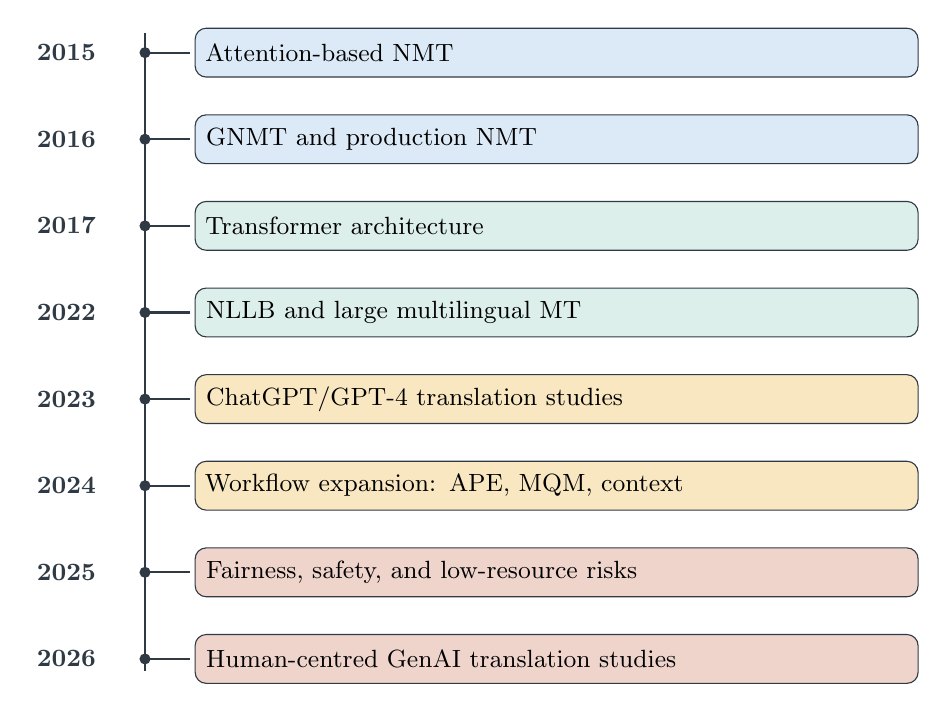
\begin{tikzpicture}[x=1cm,y=1cm,>=Latex]
\tikzstyle{milestone}=[draw=boxborder,rounded corners,align=left,text width=8.9cm,minimum height=0.62cm,font=\small,inner sep=4pt]
\newcommand{\timelinemilestone}[4]{%
\node[anchor=east,font=\bfseries\small,text=boxborder] at (0.95,#1) {#2};
\fill[boxborder] (1.45,#1) circle (2pt);
\draw[boxborder,thick] (1.45,#1) -- (2.02,#1);
\node[milestone,fill=#4,anchor=west] at (2.08,#1) {#3};
}
\draw[boxborder,thick] (1.45,0.25) -- (1.45,-7.85);
\timelinemilestone{0}{2015}{Attention-based NMT}{softblue}
\timelinemilestone{-1.1}{2016}{GNMT and production NMT}{softblue}
\timelinemilestone{-2.2}{2017}{Transformer architecture}{softgreen}
\timelinemilestone{-3.3}{2022}{NLLB and large multilingual MT}{softgreen}
\timelinemilestone{-4.4}{2023}{ChatGPT/GPT-4 translation studies}{softyellow}
\timelinemilestone{-5.5}{2024}{Workflow expansion: APE, MQM, context}{softyellow}
\timelinemilestone{-6.6}{2025}{Fairness, safety, and low-resource risks}{softred}
\timelinemilestone{-7.7}{2026}{Human-centred GenAI translation studies}{softred}
\end{tikzpicture}
\caption{Timeline from attention-based NMT to LLM-augmented translation workflows. The figure marks conceptual turning points used to frame the review rather than an exhaustive history of MT.}
\end{figure}

\subsection{Review design}
We conducted a scoping survey informed by PRISMA-ScR principles. A scoping design was chosen because the literature is heterogeneous in tasks, models, language pairs, domains, datasets, prompts, evaluation metrics, and human-participant protocols. The purpose was not to estimate a pooled effect size, but to map research activity, identify evidence clusters, and synthesize methodological gaps. The review covers work from 2017 to 2026. The start date reflects the Transformer turning point in modern NMT. The later period captures the rapid growth of ChatGPT-style and open-source LLMs in translation workflows.

\subsection{Sources, search strategy and screening}
Searches and citation chasing covered ACL Anthology, Scopus-oriented and Web of Science-oriented queries, Cambridge Core, SpringerLink, ScienceDirect, Frontiers, Wiley, SAGE, MDPI, Nature Portfolio, arXiv, and supplementary Google Scholar-style discovery. The search strategy combined MT terms with LLM and workflow terms. Queries included terms such as machine translation, neural machine translation, post-editing, MTPE, translation workflow, large language model, GPT, ChatGPT, GPT-4, Llama, Gemini, translation quality assessment, MQM, terminology, translation memory, cognitive load, trust, robustness, hallucination, low-resource, multimodal, document image, and simultaneous translation.

After pilot screening, we added targeted search lines for human translator interaction, cognitive load, trust, low-resource retrieval-augmented prompting, gender and fairness, hallucination, robustness, multimodal document translation, and enterprise translation-memory adaptation.

The formal search protocol was consolidated for the present draft on 9 June 2026. Because this is a scoping survey of a fast-moving field rather than a meta-analysis, the search combined database-style fielded strings with venue-specific and citation-chaining discovery. The complete query blocks, Scopus and Web of Science fielded strings, ACL Anthology variants, human-workflow search line, and gap-fill search lines are archived in the project search-strategy file. The screening and extraction table records the source database or discovery route, publication status, inclusion decision, workflow stage, and reproducibility notes for each record.

The search was iterative. We began with a pilot set of core records from ACL Anthology and Cambridge Core, then expanded the search in two directions. The first expansion followed model-centred terms such as large language model, GPT-4, ChatGPT, Llama, automatic post-editing, translation quality assessment, MQM, document-level translation, terminology-constrained translation, and translation memory. The second expansion targeted human-centred and risk-centred terms, including translator interaction, cognitive load, trust, professional translator, post-editor, eye-tracking, hallucination, robustness, gender bias, low-resource language, document image, simultaneous translation, and enterprise translation.

Deduplication was carried out at three levels. Exact duplicates were identified by title, DOI, and ACL Anthology identifier where available. Near duplicates were checked by comparing title variants, authors, venue information, and preprint/proceedings relationships. Conceptual overlaps were not removed when the studies had different data, tasks, evaluation methods, or workflow roles. For example, several studies evaluate ChatGPT or GPT-4 in translation, but they were retained when one addressed direct translation, another post-editing, another human evaluation, and another terminology or cognitive load. This conservative approach is appropriate for a scoping survey, because the goal is to map the range of workflow uses rather than to collapse studies into effect-size units.

Screening was first conducted at title and abstract level, then at metadata and full-text availability level where needed. Screening and coding were conducted by the author using a structured extraction sheet; uncertain cases were revisited after metadata cleanup and citation chasing rather than resolved in a single pass. Records with unstable metadata were flagged and revisited. The D011-D014 cleanup pass illustrates this procedure: publication year, author lists, proceedings status, DOI, page range, and inclusion decision were verified before the records were included in the formal extraction table. This is important because early LLM translation research often circulates as preprints, workshop papers, proceedings chapters, and ahead-of-print journal articles, and unstable metadata can otherwise distort the evidence map.

Coding used a deliberately broad extraction schema. In addition to bibliographic fields, we recorded workflow stage, model role, language pair, domain, dataset, evaluation method, human involvement, prompt reporting, code and data availability, reproducibility notes, ethics or privacy notes, and taxonomy tags. The schema was designed to support both descriptive mapping and thematic synthesis. Because many records do not report all fields, missingness itself became part of the analysis, especially for prompt reporting, participant expertise, data availability, and model versioning.

Figure 2 reports the screening flow and final extraction count.

\begin{figure}[t]
\centering
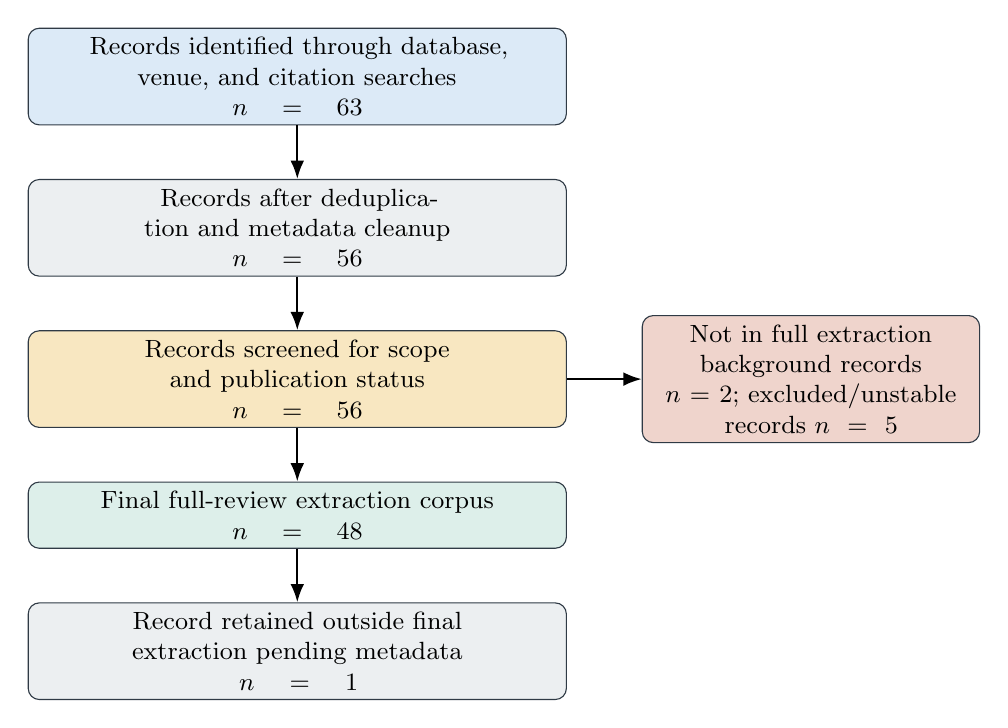
\begin{tikzpicture}[node distance=0.68cm,>=Latex]
\tikzstyle{box}=[draw=boxborder,rounded corners,align=center,text width=6.6cm,minimum height=0.78cm,fill=softblue,font=\small]
\node[box] (id) {Records identified through database, venue, and citation searches\\$n=63$};
\node[box,below=of id,fill=softgray] (dedup) {Records after deduplication and metadata cleanup\\$n=56$};
\node[box,below=of dedup,fill=softyellow] (screen) {Records screened for scope and publication status\\$n=56$};
\node[box,right=0.95cm of screen,fill=softred,text width=4.05cm] (excluded) {Not in full extraction\\background records $n=2$; excluded/unstable records $n=5$};
\node[box,below=of screen,fill=softgreen] (included) {Final full-review extraction corpus\\$n=48$};
\node[box,below=of included,fill=softgray] (pending) {Record retained outside final extraction pending metadata\\$n=1$};
\draw[->,thick] (id)--(dedup);
\draw[->,thick] (dedup)--(screen);
\draw[->,thick] (screen.east)--(excluded.west);
\draw[->,thick] (screen)--(included);
\draw[->,thick] (included)--(pending);
\end{tikzpicture}
\caption{PRISMA-style flow diagram for the final extraction corpus. The side branch separates records retained for background or journal calibration from records excluded or left outside full extraction because of scope or metadata instability. Counts reflect the project search, deduplication, metadata-cleanup, and screening logs available at the time of manuscript preparation.}
\end{figure}

\subsection{Eligibility criteria and coding}
Studies were included if they addressed MT, NMT, Transformer-based MT, LLMs, or generative AI in a substantive translation workflow. Eligible workflow stages included pre-translation support, direct translation, interactive translation, post-editing, quality estimation, quality assessment, terminology management, style control, context handling, error explanation, translator training, and workflow orchestration. Empirical studies, system papers, evaluation papers, user studies, benchmark papers, shared-task papers, and surveys were eligible. Any language pair, language direction, or domain was eligible.

Studies were excluded if they addressed general text generation, summarization, question answering, or language learning without a substantive translation component. Pure model architecture papers were excluded when they reported MT scores only as a generic benchmark and did not engage with translation workflows, evaluation practices, or applied translation technology. Non-scholarly commentary and vendor marketing materials were excluded.

Each included record was coded for bibliographic metadata, model category, model name or family, MT or NMT system, workflow stage, translation task, language pairs, domain, dataset or corpus, evaluation metrics, human evaluation, translator involvement, participant count, prompt reporting, code availability, data availability, main findings, limitations, reproducibility notes, ethics or privacy notes, and taxonomy tags. The final extraction corpus contains forty-eight full-review records, with seven additional records retained outside full extraction as background, journal-calibration, exclusion, or metadata-caution records. The formal evidence corpus includes one record from 2022, ten from 2023, twenty from 2024, fifteen from 2025, and two from 2026. ACL Anthology sources dominate the corpus, but the corpus also includes Cambridge Core, Frontiers, Nature Portfolio, Wiley, SAGE, ScienceDirect, Springer, MDPI, HiT-IT proceedings, and arXiv records.

Table 1 groups the final extraction corpus into the evidence clusters used in the synthesis.

\begin{table}[t]
\centering
\caption{Evidence clusters in the final extraction corpus. Source: authors' coding of the extraction table.}
\small
\begin{tabularx}{\textwidth}{>{\RaggedRight\arraybackslash}p{2.8cm}>{\RaggedRight\arraybackslash}p{3.5cm}>{\RaggedRight\arraybackslash}X}
\toprule
Cluster & Main workflow focus & Representative records \\
\midrule
LLM as post-editor & Revising MT or NMT output & Raunak et al. 2023; Ki and Carpuat 2024; Koneru et al. 2024; Vidal et al. 2022 \\
LLM as evaluator & Scoring, MQM-style error spans, error explanation & Kocmi and Federmann 2023a; Kocmi and Federmann 2023b; Lu et al. 2024; Lu et al. 2025; Qian et al. 2024 \\
Terminology, domain and low-resource control & Glossaries, translation memories, retrieval, fine-tuning & Moslem et al. 2023a; Moslem et al. 2023b; Berger et al. 2024; Merx et al. 2024; Court and Elsner 2024 \\
Document-level and multimodal translation & Context, literary translation, document images, multimodal data & Karpinska and Iyyer 2023; Wang et al. 2023; Wang et al. 2024; Liang et al. 2024 \\
Human-centred workflows & Cognitive load, translator expertise, post-editing behaviour & Yao et al. 2026; Chen 2025; Mau et al. 2026 \\
Fairness, robustness, hallucination and safety & Gender control, hallucination, noisy-source robustness & Lee et al. 2024; Zahraei and Emami 2025; Tang et al. 2025; Pan et al. 2024 \\
\bottomrule
\end{tabularx}
\end{table}

\section{Evidence synthesis}
\subsection{A workflow taxonomy for NMT and LLM-assisted translation}
The studies reviewed suggest that translation workflows can be organised into twelve recurring stages: pre-translation preparation; draft generation and direct translation; automatic post-editing; interactive and human-in-the-loop post-editing; terminology, style, and domain control; document-level and context-aware translation; quality estimation, translation quality assessment, and LLM-as-evaluator methods; error explanation, feedback, and evaluator-editor loops; datasets, benchmarks, and shared tasks; multi-agent and workflow orchestration; human workflow outcomes, including cognitive load, effort, productivity, trust, and expertise; and evaluation methodology, reproducibility, ethics, privacy, and professional risk.

This taxonomy highlights a key difference between NMT-centred and LLM-augmented translation. NMT systems are typically optimised as translation engines. LLMs can also act as translation engines, but much of their practical value appears in roles that are secondary or external to the engine: editing, evaluating, explaining, adapting, retrieving, and interacting. In other words, LLMs are not merely replacing one translation model with another; they are redistributing tasks across the translation pipeline.

Figure 3 visualises this redistribution of workflow roles, and Table 2 contrasts common NMT-centred and LLM-augmented patterns.

\begin{figure}[t]
\centering
\resizebox{\textwidth}{!}{%
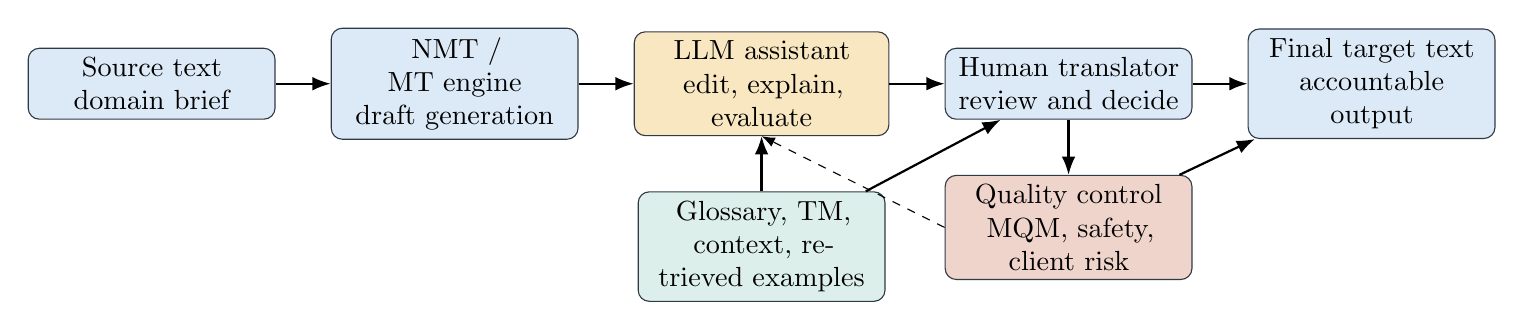
\begin{tikzpicture}[node distance=0.7cm,>=Latex]
\tikzstyle{role}=[draw=boxborder,rounded corners,align=center,text width=2.9cm,minimum height=0.9cm,fill=softblue]
\tikzstyle{llm}=[draw=boxborder,rounded corners,align=center,text width=3.0cm,minimum height=0.9cm,fill=softyellow]
\node[role] (source) {Source text\\domain brief};
\node[role,right=of source] (nmt) {NMT / MT engine\\draft generation};
\node[llm,right=of nmt] (llm) {LLM assistant\\edit, explain, evaluate};
\node[role,right=of llm] (human) {Human translator\\review and decide};
\node[role,below=of llm,fill=softgreen] (resources) {Glossary, TM, context, retrieved examples};
\node[role,below=of human,fill=softred] (qa) {Quality control\\MQM, safety, client risk};
\node[role,right=of human] (final) {Final target text\\accountable output};
\draw[->,thick] (source)--(nmt);
\draw[->,thick] (nmt)--(llm);
\draw[->,thick] (llm)--(human);
\draw[->,thick] (human)--(final);
\draw[->,thick] (resources)--(llm);
\draw[->,thick] (resources)--(human);
\draw[->,thick] (human)--(qa);
\draw[->,thick] (qa)--(final);
\draw[->,dashed] (qa.west)--(llm.south);
\end{tikzpicture}}
\caption{Workflow map of LLM-augmented translation. LLMs can be translators, post-editors, evaluators, explainers, or retrieval users; the accountable output still depends on human and institutional quality-control decisions.}
\end{figure}

\begin{table}[t]
\centering
\caption{Workflow roles of NMT and LLMs. Source: authors' synthesis.}
\small
\begin{tabularx}{\textwidth}{>{\RaggedRight\arraybackslash}p{2.7cm}>{\RaggedRight\arraybackslash}X>{\RaggedRight\arraybackslash}X}
\toprule
Workflow role & NMT-centred pattern & LLM-augmented pattern \\
\midrule
Draft generation & Task-specific MT engine produces target text & LLM may translate directly, sometimes with prompts or examples \\
Post-editing & Human or APE system revises MT output & LLM revises MT, uses error annotations, or adapts to context \\
Quality evaluation & Automatic metrics and human DA/MQM & LLM scores, explains, marks spans, or simulates evaluator roles \\
Terminology control & Glossaries, constrained decoding, TM integration & Prompts, retrieved examples, multi-agent checking, TM fine-tuning \\
Context handling & Document-level MT models and context windows & Long-context prompting, contextual refinement, discourse-aware PE \\
Human interaction & CAT tools, TM suggestions, MTPE & Conversational correction, explanation, training, trust calibration \\
\bottomrule
\end{tabularx}
\end{table}

\subsection{LLMs as post-editors of NMT output}
Automatic post-editing is one of the clearest areas in which LLMs enter translation workflows. Rather than replacing an MT system, the LLM is placed after the MT system and asked to correct, improve, or adapt its output. This design is attractive because it preserves the strengths of specialized MT systems while using LLMs for flexible revision.

Early work on LLM-based APE showed the feasibility of using large generative models to revise MT output (Vidal et al. 2022). Later work with GPT-4 found that LLMs can improve translation post-editing, but also that their behaviour depends on language pair, domain, and prompt design (Raunak et al. 2023). Ki and Carpuat (2024) showed that error annotations can guide LLMs to post-edit more effectively, linking post-editing with explicit error feedback. Koneru et al. (2024) extended the discussion to sentence-level and document-level contextual refinement, showing that context can help but also complicates evaluation.

The APE cluster reveals three design patterns. The first is direct instruction: the model is asked to improve a translation. The second is error-guided editing: the model receives error labels, MQM annotations, or human markings. The third is context-guided editing: the model receives neighbouring sentences, document context, or retrieved examples. Each pattern changes the type of evidence needed. Direct instruction can be evaluated with automatic metrics and human preferences, but error-guided and context-guided editing require finer evaluation of whether the model corrected the intended problem without introducing new errors.

Recent work also links post-editing with optimization. Huang et al. (2025) propose a reasoning-guided framework that uses multidimensional post-editing feedback to optimize LLM translation. Li et al. (2025) use monolingual data to improve document-level translation post-editing. LangMark adds a multilingual dataset for APE, which helps move the field toward more reproducible evaluation (Velazquez et al. 2025). Farrell (2023) provides a preliminary comparison of ChatGPT as both a translation engine and an automatic post-editor, showing the early uncertainty around whether ChatGPT should be treated as a direct translator, a post-editor, or both.

The main lesson is that post-editing is not a simple quality-improvement layer. It is a workflow intervention. LLM post-editors may correct errors, but they may also over-edit, change style, introduce hallucinated content, weaken terminology consistency, or obscure responsibility for the final text. Future APE research therefore needs to measure not only output quality but also edit distance, error type, terminology adherence, human revision time, and the cost of detecting LLM-introduced errors.


A key distinction in the post-editing literature is whether the LLM is asked to behave as an autonomous editor or as a constrained assistant. Autonomous editing instructions, such as asking a model to improve a translation, are easy to deploy but difficult to audit. Constrained editing, by contrast, gives the model error annotations, marked spans, terminology requirements, or retrieved examples. The latter approach is more aligned with professional translation practice because it allows the workflow to specify why an edit is needed. It also creates a clearer basis for evaluation: the question becomes whether the model corrected the marked error while preserving untouched content.

The reviewed studies also show that post-editing cannot be evaluated by aggregate quality alone. An LLM may improve fluency while weakening domain terminology, or may reduce visible grammatical errors while introducing subtle additions. In literary translation, stylistic intervention may be especially consequential because rhythm, voice, and register are part of the translation goal. In legal, medical, or technical translation, a small terminological shift can be more serious than a fluency problem. For this reason, LLM-based APE should be analysed through error-type profiles and edit operations, not only through BLEU, COMET, or human preference.

Human post-editing remains the reference point for many of these studies, but the relationship between human and LLM post-editing is not simply competitive. One emerging pattern is layered post-editing: NMT generates a draft, an LLM proposes corrections, and a human translator accepts, rejects, or revises the output. Another pattern is feedback-mediated post-editing, where human error markings are stored and later used as prompts or translation-memory-like examples. These designs suggest that the most productive question is how human feedback can make LLM post-editing more controllable and inspectable.


\subsection{LLMs as evaluators: quality estimation, MQM, and error explanation}
A second major cluster treats LLMs as evaluators of translation quality. Kocmi and Federmann (2023a) argue that LLMs can be state-of-the-art evaluators of translation quality. GEMBA-MQM extends this line by using GPT-4 to detect translation quality error spans under an MQM-style framework (Kocmi and Federmann 2023b). Other work compares LLMs for linguistic quality assessment or develops prompting methods that support human-like translation evaluation (Sinitsyna and Savenkov 2024; Lu et al. 2024).

This literature is important because evaluation is no longer a neutral afterthought. If LLMs generate translations and evaluate translations, they may also close the loop in automated pipelines. MQM-APE explicitly links error annotation prediction with automatic post-editing in LLM translation evaluators (Lu et al. 2025). Such evaluator-editor loops are attractive because they promise scalable quality control. They are also risky because they can produce self-reinforcing evaluation regimes in which the same class of model generates, judges, and revises the translation.

Human evaluation remains essential for calibration. Zhao et al. (2023) use human direct assessment to compare ChatGPT with commercial MT systems. Qian et al. (2024) ask what LLMs need for MT evaluation, drawing attention to information needs, context, and evaluation design. These studies show that LLM evaluation is not a simple replacement for human assessment. LLM evaluators may be useful for triage, explanation, or draft error annotation, but they need validation against human judgments, domain-specific criteria, and transparent protocols.

The evaluation cluster also exposes a reproducibility problem. Many LLM evaluation studies depend on proprietary models, changing model versions, undisclosed system prompts, and prompt-sensitive outputs. For an evaluator to be useful in MT research, researchers must report prompt templates, model versions, decoding settings, context windows, input formatting, and post-processing rules. Without these details, the evaluation method cannot be reliably replicated or compared.


The evaluator role deserves particular caution because it can appear more objective than it is. LLM-generated judgments are fluent and often plausible, which can make them persuasive to readers and annotators. Yet a fluent explanation is not necessarily a reliable diagnosis. The same model may be sensitive to prompt wording, ordering of candidates, presence or absence of reference translations, and whether the source sentence is shown. Some LLM evaluators may also favour outputs that resemble their own generation style. These risks are not reasons to reject LLM-based evaluation, but they are reasons to validate it carefully.

The strongest use cases for LLM evaluators may be triage and explanation rather than final adjudication. For example, an LLM can mark candidate error spans, suggest MQM categories, or generate rationales that help a human reviewer focus attention. This can reduce annotation burden if the model is calibrated and if human reviewers understand that the output is advisory. Conversely, using LLM judgments as ground truth without human validation risks replacing one expensive evaluation problem with a hidden reliability problem.

Evaluator-editor loops create another methodological issue. When an LLM evaluator identifies an error and an LLM editor revises it, the pipeline begins to resemble an automated quality-control system. This is promising for scale, but evaluation of such systems must check for error propagation. A model may repeatedly revise toward an internally preferred style, or may mask errors by producing more fluent explanations. Independent human evaluation and held-out challenge sets remain necessary.


\subsection{Terminology, style, domain, and low-resource control}
Terminology and domain control are central to professional translation. General fluency is not enough in legal, medical, technical, cultural heritage, or software localisation settings. A translation may be fluent and still fail because a key term is inconsistent, a style guide is ignored, or a local concept is flattened.

Several studies use LLMs to improve terminology handling. Moslem et al. (2023a) integrate domain terminology into MT by leveraging LLMs. Grubisic and Korencic (2025) use a metric-guided multi-agent approach for a terminology translation task. Berger et al. (2024) prompt LLMs with human error markings and similar examples from post-edited translation memories, showing how human corrections can guide later LLM corrections. Qian and Kong (2024) propose a concept-based LLM prompting and translation-memory workflow, positioning human conceptual guidance as part of machine translation.

Translation memories are especially important because they connect LLMs with existing CAT-tool infrastructures. Moslem et al. (2023b) study adaptive MT with in-context examples, fuzzy matches, and translation memories. Vieira et al. (2024) fine-tune Llama 3 8B Instruct on organization-specific translation memories and show that larger TM datasets improve in-house translation performance, while very small fine-tuning sets may degrade performance. This finding is practically important: LLM adaptation is not automatically beneficial. It depends on data volume, domain coherence, quality control, and governance.

Low-resource translation introduces additional constraints. Merx et al. (2024) use retrieval-augmented prompting for Mambai, combining dictionary entries and retrieved examples with GPT-4, Llama 2, and Mixtral. Court and Elsner (2024) study Southern Quechua-Spanish translation and show that retrieval and understanding both limit LLM performance. Mao and Yu (2024) explore contrastive alignment instructions for unseen low-resource languages. Together, these studies caution against universal claims about LLM translation. Prompting, dictionaries, and retrieved examples can help, but representative corpora, community involvement, linguistic resources, and evaluation design are decisive.

For workflow research, terminology and low-resource control should be treated together because both expose the limits of general-purpose translation. The key question is not whether an LLM can produce plausible target text. It is whether the workflow can guarantee consistent terms, respect domain constraints, support under-resourced communities, document the source of guidance, and allow human experts to inspect and correct model behaviour.


Terminology control is one of the areas where LLM flexibility is useful but also potentially dangerous. A glossary prompt may work for a short example, yet fail across a long document when terms recur in varied syntactic contexts. A translation-memory example may help style adaptation, yet introduce outdated or client-specific phrasing into a new project. A multi-agent terminology workflow may catch some inconsistencies, yet create additional complexity and cost. The question is therefore not whether LLMs can use terminology, but how terminology constraints are represented, checked, and governed across the workflow.

Enterprise translation-memory fine-tuning introduces a different set of trade-offs. Vieira et al. show that larger organization-specific translation memories can improve fine-tuned LLM translation, while very small datasets may harm performance. This result is highly relevant for practice because many organizations have uneven TM quality. Some segments are high quality and current; others are legacy translations, inconsistent revisions, or domain-specific compromises. Fine-tuning on such data can reproduce institutional terminology, but it can also amplify historical inconsistency if the TM is not curated.

Low-resource translation sharpens the ethical dimension of adaptation. Retrieval-augmented prompting with dictionaries and examples can help, as the Mambai study suggests, but the Southern Quechua study shows that retrieval and understanding remain bottlenecks. For low-resource and Indigenous languages, translation technology should not be evaluated solely by aggregate scores. Researchers need to document who created the resources, what domains they represent, what community benefit is expected, and how errors may affect speakers. Language coverage is not the same as language accountability.


\subsection{Document-level and context-aware translation}
Sentence-level MT evaluation is convenient, but many translation problems are document-level problems. Pronouns, discourse connectives, lexical cohesion, register, character voice, legal references, and terminology consistency often depend on context beyond one sentence. LLMs appear promising here because they can process longer contexts than many earlier MT pipelines.

Castilho and Knowles (2024) survey context in NMT and MT evaluation, providing an important background anchor. Karpinska and Iyyer (2023) show that LLMs can use document-level context for literary translation, but critical errors persist. Wang et al. (2023) study document-level MT with LLMs. Koneru et al. (2024) and Li et al. (2025) extend the discussion to contextual post-editing and document-level PE.

The document-level literature suggests that context is useful but not automatically safe. Longer context can help resolve ambiguity, but it can also increase the space for inconsistent or hallucinated edits. Evaluation becomes harder because sentence-level automatic metrics may miss document-level coherence problems or over-penalize acceptable contextual choices. Human evaluation protocols must therefore ask different questions: Does the translation preserve discourse coherence? Are terms consistent across the document? Does style remain stable? Are additions or omissions introduced by long-context reasoning?

Recent multimodal and document-image studies broaden the document problem. Wang et al. (2024) use LLM-based data augmentation for multimodal MT, addressing the scarcity of image-text-translation triplets. Liang et al. (2024) study document image MT with dynamic assembly of multiple pretrained models and introduce a large document-image translation dataset. These studies are not always framed as translator workflow studies, but they matter for workflow design because many real translation tasks involve PDFs, scanned documents, slides, figures, layout, or image-bound text. Document translation workflows must therefore handle not only language but also layout, modality, visual grounding, and OCR-like errors.


Document-level translation also challenges the assumption that a better model is always a larger-context model. Longer context can provide useful information, but it can also distract the model or encourage unnecessary rewriting. Context may help resolve pronouns and lexical cohesion, but it may also lead to hallucinated links between sentences. The design problem is to determine which context is useful for which decision. A neighbouring sentence, a paragraph, a document summary, a glossary, and a translation memory segment all provide different kinds of information.

Multimodal and document-image translation expand this problem beyond text. In many workflows, translators receive PDFs, scanned documents, presentations, screenshots, or image-heavy manuals. The system must recognise text, preserve layout, interpret visual context, and generate a target-language document that remains usable. Errors may arise from OCR, layout segmentation, image grounding, or translation itself. LLM-based data augmentation and dynamic pretrained model assembly are early steps toward this broader workflow, but evaluation protocols must follow. A document-image translation can be linguistically accurate and still fail if the layout makes it unusable.


\subsection{Human-centred translation workflows}
Human-centred evidence is still smaller than model-centred evidence, but it is crucial. Yao et al. (2026) examine cognitive load during AI-assisted post-editing from a cognitive ergonomics perspective. Zou et al. (2024) study syntactic complexity in LLM-leveraged post-editing involving students and expert translators. Chen (2025) uses eye-tracking to study human-machine collaborative translation. Mau et al. (2026) examine cognitive demands and translation behaviour in GenAI-assisted legal translation. Macken (2024) evaluates ChatGPT's ability to automatically post-edit literary texts, linking model performance with professional literary translation concerns.

These studies complicate the claim that AI assistance reduces effort. In some conditions, an LLM or MT system may reduce drafting time. In others, it may increase cognitive load by requiring translators to monitor plausible but wrong outputs, detect terminology drift, or decide whether to accept style changes. Assistance can become distraction when translators must constantly infer why the system produced a suggestion and whether it can be trusted.

Human expertise also changes the meaning of evaluation. Student translators, professional translators, domain experts, and general bilingual evaluators may experience the same system differently. A student may benefit from explanations but also overtrust fluent output. A professional translator may detect subtle domain errors but lose time correcting over-edits. A subject-matter expert may prioritize terminology and factuality over fluency. Workflow evaluation must therefore specify who the human is, what task they perform, what expertise they have, and what outcome is measured.

Simultaneous MT adds another human-centred dimension: latency. Wang et al. (2024) study simultaneous MT with LLMs and report advantages in some quality and latency metrics, while noting that computational cost remains a major obstacle. In live translation settings, workflow quality includes not only adequacy and fluency but also latency, robustness to noisy input, cognitive burden, and system cost.


Human-centred studies are indispensable because workflow success depends on how people use the system. Cognitive load research shows that assistance can impose monitoring costs. Eye-tracking and process data can reveal whether translators spend time reading, verifying, searching, or correcting. Corpus-based learner studies can show how student output changes after GPT-mediated post-editing. Professional literary translation studies can show whether LLM revisions respect voice and style. These outcomes are difficult to capture with standard MT metrics, but they are central to translation practice.

Trust is particularly complex. Undertrust can prevent useful adoption; overtrust can allow subtle errors to pass. The appropriate goal is calibrated trust: translators should understand where a system is strong, where it is weak, and how much verification is needed. LLM explanations may help trust calibration, but they may also create false confidence if the explanation is fluent but inaccurate. Human-centred evaluation should therefore measure not only whether users like the system, but whether they make better decisions with it.

Expertise moderates almost every workflow outcome. Students, professional translators, bilingual annotators, domain experts, and reviewers may use the same LLM output differently. A professional translator may reject unnecessary stylistic changes that a novice accepts. A domain expert may detect terminology risk that a general evaluator misses. Studies should report participant expertise in detail and avoid treating all human evaluation as equivalent.


\subsection{Fairness, robustness, hallucination, and safety}
Fairness and safety are not peripheral ethical concerns; they are translation quality concerns. A translation that misgenders a person, stereotypes a profession, hallucinates a legal condition, or fails under noisy input can cause real harm even if it appears fluent.

Gender is a rapidly developing sub-area. Lee et al. (2024) propose fine-grained gender control through entity-level prompting and identify gender interference when multiple entities are controlled. Zahraei and Emami (2025) introduce the Translate-with-Care dataset and show that GPT-4, NLLB, Google Translate, and mBART-50 struggle with genderless content, with masculine defaults and reasoning errors in some contexts. These studies show that LLMs do not automatically solve long-standing MT bias problems. Prompting can create control, but control must be evaluated across languages, morphologies, and social contexts.

Hallucination is another major risk. Tang et al. (2025) frame hallucinated translations as a trust and safety problem and propose hallucination-focused preference optimization. Their results suggest that training-time mitigation can reduce hallucinations while preserving translation quality. This is important because post-hoc hallucination detection and re-translation may add latency and complexity. However, hallucination definitions, detection methods, and high-stakes domain tests still need careful scrutiny.

Robustness to noisy input is equally practical. Pan et al. (2024) study whether LLMs can learn translation robustness from noisy-source in-context demonstrations. They find that noisy demonstrations can improve robustness in some conditions, but performance varies by noise type and setting. Real translation workflows often contain OCR errors, speech recognition errors, typographical errors, mixed-language input, informal writing, and incomplete context. Robustness should therefore be part of MT workflow evaluation rather than a secondary benchmark.


The fairness and safety cluster shows that translation quality is inseparable from social meaning. Gender control studies demonstrate that models need explicit mechanisms to handle ambiguous or genderless source content. Bias studies show that fluent translations can still reproduce stereotypes or impose gender where the source does not justify it. These problems are not merely representational; they affect identity, professional portrayal, and institutional fairness.

Hallucination is a different but equally serious failure mode. In translation, hallucination may take the form of added information, omitted constraints, invented entities, or unsupported causal relations. Because translations are often read as faithful representations of source texts, hallucinated content can be especially damaging. Preference optimization and other mitigation strategies are promising, but they must be tested across domains where hallucinations carry different risks.

Robustness connects safety to everyday noise. Real source texts contain typos, OCR artifacts, code-switching, speech recognition errors, incomplete sentences, and inconsistent formatting. If an LLM performs well on clean benchmark text but fails unpredictably on noisy input, it may be unsuitable for deployment. Robustness evaluation should therefore be built into workflow benchmarks, especially for document-image, simultaneous, and low-resource translation.

Figure 4 summarises the resulting research gaps by workflow area.

\begin{figure}[t]
\centering
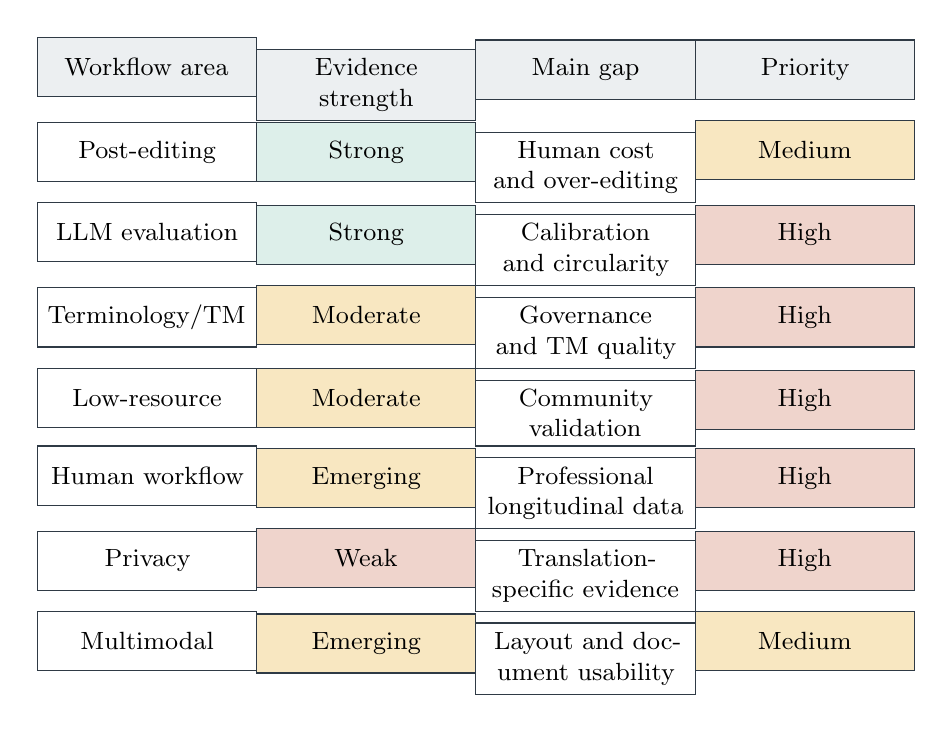
\begin{tikzpicture}[font=\small]
\matrix[matrix of nodes,nodes={draw=boxborder,minimum height=0.75cm,align=center,text width=2.55cm},column sep=-\pgflinewidth,row sep=-\pgflinewidth] (m) {
\node[fill=softgray]{Workflow area}; & \node[fill=softgray]{Evidence strength}; & \node[fill=softgray]{Main gap}; & \node[fill=softgray]{Priority}; \\
\node{Post-editing}; & \node[fill=softgreen]{Strong}; & \node{Human cost and over-editing}; & \node[fill=softyellow]{Medium}; \\
\node{LLM evaluation}; & \node[fill=softgreen]{Strong}; & \node{Calibration and circularity}; & \node[fill=softred]{High}; \\
\node{Terminology/TM}; & \node[fill=softyellow]{Moderate}; & \node{Governance and TM quality}; & \node[fill=softred]{High}; \\
\node{Low-resource}; & \node[fill=softyellow]{Moderate}; & \node{Community validation}; & \node[fill=softred]{High}; \\
\node{Human workflow}; & \node[fill=softyellow]{Emerging}; & \node{Professional longitudinal data}; & \node[fill=softred]{High}; \\
\node{Privacy}; & \node[fill=softred]{Weak}; & \node{Translation-specific evidence}; & \node[fill=softred]{High}; \\
\node{Multimodal}; & \node[fill=softyellow]{Emerging}; & \node{Layout and document usability}; & \node[fill=softyellow]{Medium}; \\
};
\end{tikzpicture}
\caption{Research gap matrix by workflow area. Colours indicate relative evidence strength and priority in the final extraction corpus.}
\end{figure}

\subsection{Evaluation practices and reproducibility}
The reviewed literature uses a wide range of evaluation methods: BLEU, chrF, TER, COMET, direct assessment, MQM, error-span annotation, lexical variety measures, eye-tracking, cognitive-load measures, Likert ratings, latency metrics, and qualitative translator behaviour analysis. Each captures a different part of workflow quality.

Automatic metrics remain useful for scale, especially in system comparisons and dataset studies. However, they are limited when the research question concerns terminology, style, document coherence, cognitive effort, or safety. Human evaluation is indispensable, but it must be reported in detail. Many studies still need clearer information about evaluator expertise, recruitment, annotation instructions, agreement, payment, language competence, and domain knowledge.

LLM-based evaluation adds a new reproducibility burden. A study that uses GPT-4 or another proprietary model as an evaluator should report the model version, date of access, prompt, context, decoding settings, and any post-processing. If the model is updated silently, later replication may not produce the same results. For open-source models, researchers should report model checkpoints, inference settings, hardware constraints, and any fine-tuning or retrieval configuration.

Data and code availability are uneven. Some benchmark and dataset papers provide resources, while many prompt-based workflow papers do not provide full prompt templates, source segments, MT outputs, or human annotations. This weakens cumulative research. For a workflow-oriented field, reproducibility should include not only model and data, but also task instructions, CAT-tool context, translation memories, glossaries, and evaluation rubrics.

Table 3 proposes a minimum reporting checklist for future LLM-augmented MT workflow studies.

\begin{table}[t]
\centering
\caption{Minimum reporting checklist for LLM-augmented MT workflow studies. Source: authors' synthesis.}
\small
\begin{tabularx}{\textwidth}{>{\RaggedRight\arraybackslash}p{2.7cm}>{\RaggedRight\arraybackslash}X}
\toprule
Category & Minimum reporting item \\
\midrule
Model & Model family, version, access date, checkpoint, decoding settings \\
Prompting & Full prompt template, examples, system instructions, context window \\
Translation resources & Source texts, MT outputs, references, glossaries, translation memories \\
Human participants & Expertise, language profile, task role, recruitment, consent, compensation \\
Evaluation & Metrics, rubrics, annotation protocol, agreement, error taxonomy \\
Reproducibility & Code, data, prompts, model settings, random seeds where applicable \\
Risk & Privacy, confidentiality, hallucination, bias, domain safety considerations \\
\bottomrule
\end{tabularx}
\end{table}


\section{Discussion and research agenda}
\subsection{Cross-cluster synthesis: what changes when translation is treated as a workflow}
The preceding sections separate the evidence into analytical clusters, but the most important implications appear at the boundaries between clusters. LLM-based post-editing, LLM-based evaluation, terminology control, document-level context, human-centred outcomes, and safety risks are not independent topics. They interact in ways that define the practical value of LLM-augmented translation. A post-editor that improves fluency may create evaluation problems if the evaluator is also an LLM. A terminology workflow that uses retrieved examples may create privacy risks if the examples come from client translation memories. A document-level context method may improve cohesion while increasing the risk of hallucinated discourse links. A simultaneous MT system may score well on BLEU and latency while still being unusable if the computational cost is too high or if noisy input produces unstable output. The workflow view makes these interactions visible.

The first cross-cluster finding is that LLMs are strongest when the task can be decomposed into inspectable subtasks. Direct translation asks the model to solve all problems at once: understand the source, infer context, choose terminology, produce fluent target text, and maintain style. Workflow designs can distribute those responsibilities. An NMT system can generate an initial draft; a glossary or translation memory can provide constraints; an LLM can propose edits or explanations; a human translator can decide; and an evaluation stage can check for adequacy, terminology, fairness, and safety. This decomposition does not remove error, but it creates opportunities for diagnosis. If a term is wrong, the workflow can ask whether the glossary was absent, the retrieval failed, the LLM ignored the constraint, or the human reviewer accepted a bad suggestion. Without decomposition, the failure is simply attributed to the model.

The second finding is that LLM value often depends on the availability of external structure. The strongest workflow uses are rarely unconstrained prompting alone. Error annotations, MQM labels, human markings, translation memories, dictionaries, glossaries, document context, and retrieved examples all provide structure that makes LLM behaviour more targetable. This pattern cuts across post-editing, terminology, low-resource translation, and evaluation. It also suggests that future progress may come less from asking whether the newest model is better and more from asking what information the model needs, how that information should be represented, and how the workflow verifies that the information was used correctly.

The third finding is that evaluation has to become multi-layered. A single metric cannot evaluate a workflow. Automatic MT metrics can compare output strings, but they cannot fully capture whether a translator had to spend extra effort monitoring an LLM suggestion, whether a glossary was consistently applied across a document, whether a gender-neutral source was translated fairly, or whether a model hallucinated a legal obligation. Human evaluation can address some of these questions, but only if the protocol specifies evaluator expertise and decision criteria. Process measures such as eye-tracking, keystrokes, time-on-task, edit distance, and cognitive-load scales add another layer. Risk-specific evaluations for hallucination, bias, noisy input, privacy, and toxicity add yet another. A mature evaluation design will combine these layers rather than choosing one.

The fourth finding is that the role of the human translator is becoming more differentiated. In early MTPE research, the human was often treated as a post-editor who corrected machine output. In LLM-augmented workflows, the human may also be a prompt designer, terminology curator, error marker, quality judge, domain expert, trainer, or final accountable author of the translation. These roles require different expertise and create different burdens. A translator asked to mark errors for a self-correcting MT workflow is doing data work as well as translation work. A translator asked to evaluate LLM explanations is doing epistemic quality control. A translator asked to use an LLM in legal translation must manage not only text quality but also confidentiality, liability, and client trust.

This differentiation matters for study design. It is no longer enough to report that human evaluators were used. Researchers should specify whether humans translated, post-edited, ranked outputs, annotated MQM errors, provided error markings, supplied reference translations, judged cognitive load, or validated low-resource language outputs. They should also specify whether those humans were students, professional translators, bilingual speakers, domain experts, or trained annotators. Without these details, human-centred claims remain difficult to interpret.

The fifth finding is that LLM workflows intensify the need for governance. Traditional MT workflows already required decisions about data, terminology, and responsibility. LLMs add new governance questions: Can client text be sent to an external API? Can translation memories be used for fine-tuning? Who approves prompt templates? How are model updates tracked? Who is responsible if an LLM evaluator misses an error introduced by an LLM post-editor? What happens when a model explanation conflicts with a human translator's judgement? These questions are not external to NLP research. They determine whether a method can be responsibly deployed.

The sixth finding is that low-resource and high-stakes settings should not be treated as edge cases. They are stress tests for the assumptions behind LLM translation. Low-resource languages reveal whether a system can use dictionaries, grammars, retrieved examples, and community data without overclaiming competence. Legal and medical domains reveal whether fluency can coexist with terminological precision and risk control. Gender-sensitive translation reveals whether models can preserve social meaning rather than imposing defaults. Document-image and simultaneous translation reveal whether models remain reliable when the input is noisy, multimodal, or time-constrained. If a workflow only works for clean high-resource benchmark text, its practical contribution is narrower than its headline may suggest.

The seventh finding concerns the relationship between closed and open models. Proprietary models such as GPT-4 have driven much of the early LLM translation literature because they are strong, accessible through APIs, and easy to prompt. Open models are increasingly important for reproducibility, privacy, local deployment, and low-resource experimentation. The workflow perspective does not imply that one class is always preferable. Instead, it asks what the workflow requires. A research prototype may use a closed model for exploratory evaluation; a confidentiality-sensitive translation workflow may require a local model; a low-resource community project may prefer open models that can be inspected and adapted; a large enterprise workflow may combine API models, local models, and translation memories under governance constraints. Reporting should make these choices explicit.

The final cross-cluster implication is that the field needs to stop treating prompt engineering as an informal detail. Prompts are now part of the method. They define the role of the LLM, the task constraints, the expected output format, and sometimes the evaluation rubric. In translation workflows, a prompt may encode terminology instructions, style preferences, privacy warnings, error categories, or human feedback. If prompts are not reported, the study cannot be replicated. If prompts are changed during experimentation without documentation, the reported performance cannot be interpreted. Prompt reporting should therefore be treated like dataset reporting or model reporting.

Taken together, these cross-cluster findings support the main thesis of this survey. LLMs are not simply new MT systems. They are flexible components that can be placed into translation workflows in multiple roles. That flexibility is the source of their promise and the source of their risk. The most useful future work will be precise about role, constraint, evidence, human involvement, and accountability.


\subsection{Implications for NLP research}
The workflow view has several implications for NLP as a field. First, it suggests that translation should remain a central testbed for evaluating general-purpose language models. MT is not only a benchmark of multilingual generation; it is a task where semantic fidelity, discourse context, domain terminology, social meaning, and human accountability all matter at the same time. A model that performs well on open-ended generation may still fail as a translation assistant if it cannot preserve source constraints or make its revisions inspectable. Conversely, a model that is not the strongest direct translator may still be useful as an evaluator, terminology checker, or post-editing assistant.

Second, the findings support a more modular view of NLP systems. Much recent discussion of LLMs emphasises end-to-end prompting, but translation workflows show the value of modular composition. A retrieval component can supply terminology or examples. A specialised NMT model can produce a draft. An LLM can revise or explain. A human translator can adjudicate. A risk checker can flag hallucination, gender bias, or confidentiality concerns. This modular view is not a retreat from LLMs; it is a way of making them more accountable. It also fits broader NLP trends toward tool use, retrieval augmentation, agents, and human-in-the-loop systems.

Third, translation workflows reveal a tension between benchmark progress and situated usefulness. Benchmarks are essential for comparing systems, but they tend to simplify the task. They often remove client-specific terminology, confidential data, long documents, inconsistent translation memories, formatting constraints, and human revision. Real workflows reintroduce these conditions. NLP research should therefore develop benchmarks that simulate workflow complexity without sacrificing reproducibility. Such benchmarks might include a source document, an NMT draft, a glossary, a translation memory fragment, an LLM prompt, a human revision trace, and an error annotation protocol.

Fourth, the survey highlights the importance of model documentation and temporal stability. LLM translation studies often depend on API-based models that change over time. If the model version is unclear, a later researcher may not be able to reproduce the result. This is especially problematic when the LLM is used as an evaluator. NLP venues should encourage authors to report not only the model name but also the exact version, access date, decoding settings, prompt, and any system instruction. Where exact reproducibility is impossible, authors should state the limitation explicitly.

Fifth, workflow-centred MT can contribute to responsible NLP. Fairness, hallucination, privacy, and low-resource language equity are often discussed as broad AI ethics topics. Translation turns them into concrete engineering and evaluation problems. A gender-biased translation can be observed and counted. A hallucinated clause can be compared against a source text. A low-resource translation can be validated by community speakers. A confidentiality risk can be traced through an API call or fine-tuning pipeline. This concreteness makes translation a valuable domain for developing responsible NLP methods that are empirically testable.

Finally, the survey suggests that NLP research should take professional expertise seriously. Translators are not merely end users of MT systems; they are knowledge workers who manage meaning, risk, style, and accountability. Their interaction with LLMs can produce data, corrections, prompts, and evaluation judgments that improve systems. But this interaction has a cost. If NLP systems rely on human expertise, studies should measure and value that expertise rather than treating it as invisible labour. Workflow evaluation is therefore also labour evaluation.

The implication is practical as well as theoretical. If translation is used as a benchmark for multilingual intelligence, researchers should report whether the model is being evaluated as a translator, an editor, an evaluator, or a workflow participant. These roles draw on overlapping capabilities, but they create different risks. A strong editor can be a poor final judge; a good evaluator can be too expensive for real-time use; a helpful explanation can still be wrong. Separating these roles will make NLP claims clearer and will make translation research more useful for practitioners.

\subsection{Open challenges}
Five challenges stand out. First, professional deployment evidence remains thin. Many studies use benchmark datasets, short texts, or laboratory tasks. Fewer examine real CAT-tool workflows, client constraints, translation-memory governance, confidentiality, revision cycles, or longitudinal adoption.

Second, privacy and confidentiality are underdeveloped in translation-specific research. Professional translation often involves sensitive legal, medical, financial, or institutional data. General LLM privacy discussions are relevant, but translation workflows need domain-specific evidence about what data enters external models, how it is stored, and who is accountable.

Third, human-centred outcomes are not yet standard. Cognitive load, trust, effort, productivity, and expertise should not be occasional add-ons. They are central to whether LLM assistance is useful. A translation workflow that improves COMET but increases translator monitoring burden may not be a better workflow.

Fourth, low-resource and culturally specific translation remains fragile. Retrieval and prompting can help, but the evidence shows that language-community data, representative test sets, and human involvement matter. LLM translation research should avoid treating low-resource languages as merely difficult benchmark conditions.

Fifth, evaluation loops can become circular. If LLMs translate, evaluate, explain, and post-edit, then model-family biases may be reinforced. Human evaluation, transparent rubrics, and independent error analysis are needed to prevent closed-loop overconfidence.


The privacy gap is especially important for translation. Translators frequently handle unpublished manuscripts, contracts, medical records, immigration documents, litigation materials, internal corporate reports, and culturally sensitive community texts. Sending such material to a third-party LLM may breach contractual or legal obligations. Yet many technical studies treat input text as a neutral benchmark object. Future work should specify whether data can be sent to external APIs, whether local models are required, and how translation memories are protected.

Another challenge is the lack of longitudinal evidence. A system that looks useful in a short experiment may change work practices over months. Translators may become more efficient, or they may become dependent on suggestions. They may develop better error-detection strategies, or they may become less attentive to routine segments. Longitudinal workplace studies would help distinguish novelty effects from durable workflow value.

Finally, the field needs better negative evidence. Publication incentives favour improvements, but workflow research also needs to know when LLMs fail, when they increase effort, when small fine-tuning sets harm performance, when prompts do not transfer, and when human reviewers reject LLM suggestions. Such evidence is not a weakness of the field; it is the material from which reliable guidance is built.


\subsection{Research agenda}
Future research should move in six directions. First, build workflow benchmarks rather than only output benchmarks. Such benchmarks should include source text, MT output, LLM suggestions, human edits, terminology constraints, time logs, and final quality judgments. They should also include negative cases, because a workflow benchmark that contains only successful examples will encourage unrealistic claims.

Second, evaluate LLMs in CAT-tool-like settings. Researchers should study how translators interact with LLM suggestions, explanations, and revisions inside realistic workflows, including translation memories, glossaries, and client style guides. This includes measuring the time required to inspect suggestions and the error types that escape detection.

Third, make reproducibility a first-class contribution. Prompt templates, model versions, evaluation rubrics, and extracted resources should be released whenever legally possible. When release is impossible, researchers should provide synthetic or redacted equivalents. Reproducibility should extend to human protocols, including task instructions and annotation guidelines.

Fourth, integrate fairness, hallucination, and robustness into standard MT evaluation. Gender control, reasoning consistency, noisy-source robustness, and hallucination should be reported alongside adequacy and fluency in LLM-augmented MT studies. These dimensions should be treated as translation quality dimensions, not separate ethical appendices.

Fifth, design low-resource research with community involvement. Retrieval, dictionaries, and prompting should be paired with careful corpus documentation, native-speaker validation, and transparent discussion of community benefit and risk. Researchers should be especially cautious about claiming coverage or competence for languages where evaluation data are narrow.

Sixth, separate roles in evaluation. Studies should distinguish when an LLM is the translator, post-editor, evaluator, explainer, or data generator. Combining these roles may be useful, but it should be explicitly justified and independently validated. Role separation will make it easier to diagnose where a workflow succeeds or fails.

\section{Conclusion}
The literature reviewed in this survey shows that LLMs are changing machine translation less as isolated replacement engines and more as workflow components. They post-edit NMT output, evaluate quality, generate MQM-style explanations, retrieve and apply terminology, incorporate translation memories, handle document context, support low-resource prompting, augment multimodal data, and interact with human translators. This makes translation an important test case for human-centred and workflow-centred NLP.

The field's main challenge is therefore not simply to determine whether LLMs translate better than NMT systems. The harder question is whether LLM-augmented workflows are reliable, reproducible, cognitively ergonomic, terminology-aware, fair, safe, and accountable. Answering that question will require stronger reporting standards, more professional workflow studies, deeper low-resource collaboration, and evaluation designs that measure both text quality and human work.

A workflow view also changes how survey claims should be read. The evidence does not support a simple conclusion that LLMs replace NMT, nor does it support the opposite claim that LLMs are merely unreliable generalists. Instead, it shows that LLMs are useful when their role is specified, their constraints are explicit, and their outputs are evaluated in relation to human and institutional goals. The next phase of MT research should therefore be less concerned with isolated demonstrations of impressive translation and more concerned with building accountable translation workflows.

For journal readers, this distinction is useful because it prevents a common overgeneralisation. A single LLM translation score does not tell us whether the system is suitable for translator training, legal post-editing, low-resource community work, or enterprise localisation. Each use case asks for a different balance of quality, cost, transparency, privacy, and human control.

\section*{Acknowledgements}
No non-author acknowledgements are declared in this pre-submission draft. Use of artificial intelligence tools: AI tools were used to assist with literature organisation, screening support, data extraction structuring, figure drafting, LaTeX preparation, and manuscript drafting. The authors reviewed, revised, and remain responsible for all content, claims, citations, and interpretations.

\section*{Author contribution statement}
Xiongfei Wang is responsible for conceptualisation, methodology, literature search, screening, data extraction, formal analysis, visualisation, writing -- original draft, and writing -- review and editing.

\section*{Competing interests}
The authors declare no competing interests.

\section*{Funding}
This work was supported by the 2024 Postgraduate Research and Innovation Projects at Guangdong University of Foreign Studies under the project \emph{Metaphor Interpretation and Translation of Large Language Models} (Grant No. 24GWCXXM-016).

\section*{Data availability statement}
The screening records, search strategy, evidence map, codebook, metadata-cleanup notes, and PRISMA-style count documentation supporting this survey are available in Zenodo at \url{https://doi.org/10.5281/zenodo.20645622}. The corresponding GitHub repository is available at \url{https://github.com/Nighthme/llm-translation-workflow-survey}.

\section*{Ethics statement}
Ethical approval was not required for this scoping survey because it analyses published literature and does not report new research involving human participants, human tissue, or non-public personal data.

\section*{References}
\footnotesize
\RaggedRight
Ataman, D., Birch, A., Habash, N., Federico, M., Koehn, P. and Cho, K. (2025). Machine translation in the era of large language models: a survey of historical and emerging problems. \emph{Information} 16(9), 723. doi:10.3390/info16090723.

Bahdanau, D., Cho, K. and Bengio, Y. (2015). Neural machine translation by jointly learning to align and translate. In \emph{International Conference on Learning Representations}.

Berger, N., Riezler, S., Exel, M. and Huck, M. (2024). Prompting large language models with human error markings for self-correcting machine translation. In \emph{Proceedings of the 25th Annual Conference of the European Association for Machine Translation}, 636--646.

Castilho, S. and Knowles, R. (2024). A survey of context in neural machine translation and its evaluation. \emph{Natural Language Processing}. Cambridge Core article 875C3E2DEAAB8845A0F05988D5A18B55.

Chen, L. (2025). Examining cognitive load in human-machine collaborative translation: insights from eye-tracking experiments of Chinese-English translation. \emph{Frontiers in Psychology} 16. doi:10.3389/fpsyg.2025.1570929.

Court, S. and Elsner, M. (2024). Shortcomings of LLMs for low-resource translation: retrieval and understanding are both the problem. In \emph{Proceedings of the Ninth Conference on Machine Translation}, 1332--1354. doi:10.18653/v1/2024.wmt-1.125.

Farrell, M. (2023). Preliminary evaluation of ChatGPT as a machine translation engine and as an automatic post-editor of raw machine translation output from other machine translation engines. In \emph{Proceedings of the International Conference HiT-IT 2023}, 108--113. doi:10.26615/issn.2683-0078.2023\_009.

Grubisic, I. and Korencic, D. (2025). IRB-MT at WMT25 terminology translation task: metric-guided multi-agent approach. In \emph{Proceedings of the Tenth Conference on Machine Translation}, 1302--1334. doi:10.18653/v1/2025.wmt-1.110.

Huang, Y., Zang, X., Ji, C. and Chen, Z. (2025). Reasoning-guided LLM translation optimization: a framework using multidimensional postediting feedback. \emph{International Journal of Intelligent Systems} 2025(1), 9971702. doi:10.1155/int/9971702.

Karpinska, M. and Iyyer, M. (2023). Large language models effectively leverage document-level context for literary translation but critical errors persist. In \emph{Proceedings of the Eighth Conference on Machine Translation}, 419--451. doi:10.18653/v1/2023.wmt-1.41.

Ki, D. and Carpuat, M. (2024). Guiding large language models to post-edit machine translation with error annotations. In \emph{Findings of the Association for Computational Linguistics: NAACL 2024}. doi:10.18653/v1/2024.findings-naacl.265.

Kocmi, T. and Federmann, C. (2023a). Large language models are state-of-the-art evaluators of translation quality. In \emph{Proceedings of the 24th Annual Conference of the European Association for Machine Translation}.

Kocmi, T. and Federmann, C. (2023b). GEMBA-MQM: detecting translation quality error spans with GPT-4. In \emph{Proceedings of the Eighth Conference on Machine Translation}. doi:10.18653/v1/2023.wmt-1.64.

Koneru, S., Exel, M., Huck, M. and Niehues, J. (2024). Contextual refinement of translations: large language models for sentence and document-level post-editing. In \emph{Proceedings of NAACL 2024: Human Language Technologies}. doi:10.18653/v1/2024.naacl-long.148.

Lee, M., Koh, H., Kim, M. and Jung, K. (2024). Fine-grained gender control in machine translation with large language models. In \emph{Proceedings of NAACL 2024: Human Language Technologies}, 5416--5430. doi:10.18653/v1/2024.naacl-long.303.

Li, Z., Rao, Z., Shang, H., Guo, J., Li, S., Wei, D. and Yang, H. (2025). Enhancing large language models for document-level translation post-editing using monolingual data. In \emph{Proceedings of COLING 2025}.

Liang, Y., Zhang, Y., Ma, C., Zhang, Z., Zhao, Y., Xiang, L., Zong, C. and Zhou, Y. (2024). Document image machine translation with dynamic multi-pre-trained models assembling. In \emph{Proceedings of NAACL 2024: Human Language Technologies}, 7084--7095. doi:10.18653/v1/2024.naacl-long.392.

Lu, Q., Qiu, B., Ding, L., Zhang, K., Kocmi, T. and Tao, D. (2024). Error analysis prompting enables human-like translation evaluation in large language models. In \emph{Findings of the Association for Computational Linguistics: ACL 2024}, 8801--8816. doi:10.18653/v1/2024.findings-acl.520.

Lu, Q., Ding, L., Zhang, K., Zhang, J. and Tao, D. (2025). MQM-APE: toward high-quality error annotation predictors with automatic post-editing in LLM translation evaluators. In \emph{Proceedings of the 31st International Conference on Computational Linguistics}, 5570--5587.

Macken, L. (2024). Machine translation meets large language models: evaluating ChatGPT's ability to automatically post-edit literary texts. In \emph{Proceedings of the 1st Workshop on Creative-text Translation and Technology}, 65--81.

Mao, Z. and Yu, Y. (2024). Tuning LLMs with contrastive alignment instructions for machine translation in unseen, low-resource languages. In \emph{Proceedings of the Seventh Workshop on Technologies for Machine Translation of Low-Resource Languages}, 1--25. doi:10.18653/v1/2024.loresmt-1.1.

Mau, B.-R., Wu, Y.-P. and Feng, H.-H. (2026). Mind the cognitive load gap: student translators' cognitive demands and translation behaviors in GenAI-assisted legal translation. \emph{System} 139, 104033. doi:10.1016/j.system.2026.104033.

Merx, R., Mahmudi, A., Langford, K., de Araujo, L. A. and Vylomova, E. (2024). Low-resource machine translation through retrieval-augmented LLM prompting: a study on the Mambai language. In \emph{Proceedings of EURALI at LREC-COLING 2024}, 1--11.

Moslem, Y., Romani, G., Molaei, M., Kelleher, J. D., Haque, R. and Way, A. (2023a). Domain terminology integration into machine translation: leveraging large language models. In \emph{Proceedings of the Eighth Conference on Machine Translation}. doi:10.18653/v1/2023.wmt-1.82.

Moslem, Y., Haque, R., Kelleher, J. D. and Way, A. (2023b). Adaptive machine translation with large language models. In \emph{Proceedings of the 24th Annual Conference of the European Association for Machine Translation}, 227--237.

NLLB Team, Costa-jussa, M. R. et al. (2024). Scaling neural machine translation to 200 languages. \emph{Nature}. doi:10.1038/s41586-024-07335-x.

Pan, L., Leng, Y. and Xiong, D. (2024). Can large language models learn translation robustness from noisy-source in-context demonstrations? In \emph{Proceedings of LREC-COLING 2024}, 2798--2808.

Qian, M. and Kong, C. (2024). Enabling human-centered machine translation using concept-based large language model prompting and translation memory. In \emph{Artificial Intelligence in HCI: HCII 2024 Proceedings, Part III}, 118--134.

Qian, S., Sindhujan, A., Kabra, M., Kanojia, D., Orasan, C., Ranasinghe, T. and Blain, F. (2024). What do large language models need for machine translation evaluation? In \emph{Proceedings of EMNLP 2024}. doi:10.18653/v1/2024.emnlp-main.214.

Raunak, V., Sharaf, A., Wang, Y., Awadalla, H. and Menezes, A. (2023). Leveraging GPT-4 for automatic translation post-editing. In \emph{Findings of the Association for Computational Linguistics: EMNLP 2023}. doi:10.18653/v1/2023.findings-emnlp.804.

Seamless Communication et al. (2025). Joint speech and text machine translation for up to 100 languages. \emph{Nature}. doi:10.1038/s41586-024-08359-z.

Sinitsyna, D. and Savenkov, K. (2024). Comparative evaluation of large language models for linguistic quality assessment in machine translation. In \emph{Proceedings of the 16th Conference of the Association for Machine Translation in the Americas}, 154--183.

Tang, Z., Chatterjee, R. and Garg, S. (2025). Mitigating hallucinated translations in large language models with hallucination-focused preference optimization. In \emph{Proceedings of NAACL 2025: Human Language Technologies}, 3410--3433. doi:10.18653/v1/2025.naacl-long.175.

Vaswani, A., Shazeer, N., Parmar, N., Uszkoreit, J., Jones, L., Gomez, A. N., Kaiser, L. and Polosukhin, I. (2017). Attention is all you need. In \emph{Advances in Neural Information Processing Systems 30}.

Velazquez, D., Grace, M., Karageorgos, K., Carin, L., Schliem, A., Zaikis, D. and Wechsler, R. (2025). LangMark: a multilingual dataset for automatic post-editing. In \emph{Proceedings of ACL 2025}. doi:10.18653/v1/2025.acl-long.1569.

Vidal, B., Llorens, A. and Alonso, J. (2022). Automatic post-editing of MT output using large language models. In \emph{Proceedings of the 15th Biennial Conference of the Association for Machine Translation in the Americas (Volume 2: Users and Providers Track and Government Track)}, 84--106.

Vieira, I., Allred, W., Lankford, S., Castilho, S. and Way, A. (2024). How much data is enough data? Fine-tuning large language models for in-house translation: performance evaluation across multiple dataset sizes. In \emph{Proceedings of the 16th Conference of the Association for Machine Translation in the Americas}, 236--249.

Wang, L., Lyu, C., Ji, T., Zhang, Z., Yu, D., Shi, S. and Tu, Z. (2023). Document-level machine translation with large language models. In \emph{Proceedings of EMNLP 2023}. doi:10.18653/v1/2023.emnlp-main.1036.

Wang, M., Vu, T.-T., Zhao, J., Shiri, F., Shareghi, E. and Haffari, G. (2024). Simultaneous machine translation with large language models. In \emph{Proceedings of the 22nd Annual Workshop of the Australasian Language Technology Association}, 89--103.

Wang, Y., Li, D., Shen, J., Xu, Y., Xu, M., Funakoshi, K. and Okumura, M. (2024). LAMBDA: large language model-based data augmentation for multi-modal machine translation. In \emph{Findings of the Association for Computational Linguistics: EMNLP 2024}, 15240--15253. doi:10.18653/v1/2024.findings-emnlp.893.

Wu, Y., Schuster, M., Chen, Z., Le, Q. V., Norouzi, M., Macherey, W., Krikun, M. et al. (2016). Google's neural machine translation system: bridging the gap between human and machine translation. arXiv:1609.08144.

Yao, Y., Han, T. and Li, D. (2026). Assistance or distraction? A cognitive ergonomics perspective on cognitive load during AI-assisted post-editing. \emph{International Journal of Human-Computer Interaction}, 1--20. doi:10.1080/10447318.2026.2628994.

Zahraei, P. S. and Emami, A. (2025). Translate with care: addressing gender bias, neutrality, and reasoning in large language model translations. In \emph{Findings of the Association for Computational Linguistics: ACL 2025}, 476--501. doi:10.18653/v1/2025.findings-acl.26.

Zhao, Y., Zhang, M., Chen, X., Deng, Y., Geng, A., Liu, L., Liu, X. et al. (2023). Human evaluation for translation quality of ChatGPT: a preliminary study. In \emph{Proceedings of the International Conference HiT-IT 2023}, 282--287. doi:10.26615/issn.2683-0078.2023\_023.

Zou, L., Carl, M., Momtaz, S. and Mirzapour, M. (2024). Impact of syntactic complexity on the processes and performance of large language models-leveraged post-editing. In \emph{Proceedings of the 16th Conference of the Association for Machine Translation in the Americas (Volume 2: Presentations)}, 259--260.

\end{document}
